\chapter{基于弱标签的语义分割}
% 在本文中,我们提出了一种新的三维物体分割的弱监督学习策略,以解决上述的挑战。我们的主要想法包括两个方面。首先,我们提出了一种自学习方法,通过物体样本增强的方法,来捕捉目标物体类别的三维形状先验。随后,我们将这种学习到的形状先验纳入具有形状感知的分割网络的训练过程。另外,我们采用了一个稀疏的弱标注方案,以更好地利用物体掩膜的空间连续性,并在不增加整体标注成本的情况下促进形状上下文的学习。
%为了实现这一目标,我们设计了一个由两个主要模块组成的深度神经网络:一个是标准的语义分割网络,它从三维输入图像中产生一个初始的三维分割掩膜;另一个是形状去噪网络,它对初始分割掩膜进行改进并输出一个最终的三维分割。为了训练深度网络,我们首先引入一种稀疏的弱标注方案,在该方案中,我们只标注三维数据的一个特定的二维图像切片的子集(可以将三维图像数据视作一系列连续的二维图像切片),同时对每张二维图像,我们设计了一种混合式弱标签,它结合了前景涂鸦和目标物体的一个宽松边界框。给定这样的弱标注形式,我们为前述的网络模型设计了一个迭代学习框架,交替进行像素级标签生成和网络参数更新。

在本章,我们为基于弱标签的语义分割提出一种新的结合形状先验的学习策略。我们的目标是利用物体的形状先验设计更有效的弱监督分割框架,并将其纳入训练过程。为此,我们探索自学习方法,从仅有弱标签的训练数据中学到目标类别的形状先验。更进一步,我们对比了不同的弱标注策略,并提出一种新的混合式标注方法,来为弱监督学习提供更有效的训练信息和更好的性能。我们采用了迭代学习的方法,来逐步地提升分割效果,直至模型参数收敛。

% 各小节介绍
本章分为以下五个部分。在第一节我们对基于弱标签的语义分割任务进行介绍,第二节介绍我们提出的结合形状先验的弱监督分割模型。然后,在第三节我们提出新的高效的稀疏弱标注策略,随后在第四节详细介绍了模型的训练方法,特别是自学习形状模型的策略。第五节为实验部分,包括实验设置、实验细节、定量结果、定性结果、消融实验等。最后一节是本章总结。

\section{问题概述}
医学图像的分割任务如图~\ref{c3_fig1}所示,左侧为二维图像及其分割结果,右侧为三维图像及其三维分割可视化(三维图像由一系列连续的二维图像堆叠成统一的整体)。
特别地是,基于弱标签的语义分割,其训练样本采用了弱标签而非全标签的形式。
给定一个输入的三维体积图像 $\mathbf{I} \in \mathbb{R}^{H \times W \times D}$,我们的目标是估计其分割掩膜 $\mathbf{M} \in \mathcal{S}^{H \times W \times D}$,其中 $H$ and $W$ 是图像切片的高度和宽度,$D$ 则是组成三维图像的切片数目。$\mathcal{S} = \{0, 1\}$ 是语义标签集,其中 $0$ 表示背景类,$1$ 为前景类。
训练数据集 $\mathcal{D} = \{\mathbf{I}^n, \mathbf{Y}^n\}_{n=1}^N$,其中 $\mathbf{Y}^n \in \mathcal{S}'^{H \times W \times D}$ 是 $\mathbf{I}^n$ 对应的弱标签, $\mathcal{S}' = \mathcal{S} \cup \{u\}$ 且 $u$ 代表无标签像素,$N$ 是训练数据样本的数目。
在本文中,我们关注二分类分割问题,即只有前景类别和背景类别。我们的方法可以通过单独处理每个类别来应用在多分类问题。

这个工作中我们的核心思想是,从弱标签中得到一个自学习的形状先验,然后利用这个形状先验来进一步进行形状去噪和改进。为了实现这一目标,我们设计了一个由两个主要模块组成的深度神经网络:一个语义分割模块和一个形状去噪模块。我们首先用语义分割模块在输入图像上预测一个初始的粗分割掩膜,然后形状去噪模块在初始掩膜上应用自学习的形状先验来进行去噪和改进。为了进一步利用形状先验来改进模型,我们采用了一种迭代学习框架,它在生成伪标签和更新模型参数之间迭代进行。我们的模型概览见图~\ref{fig:model}。


    \begin{figure*}[tbp]
        \centering 
        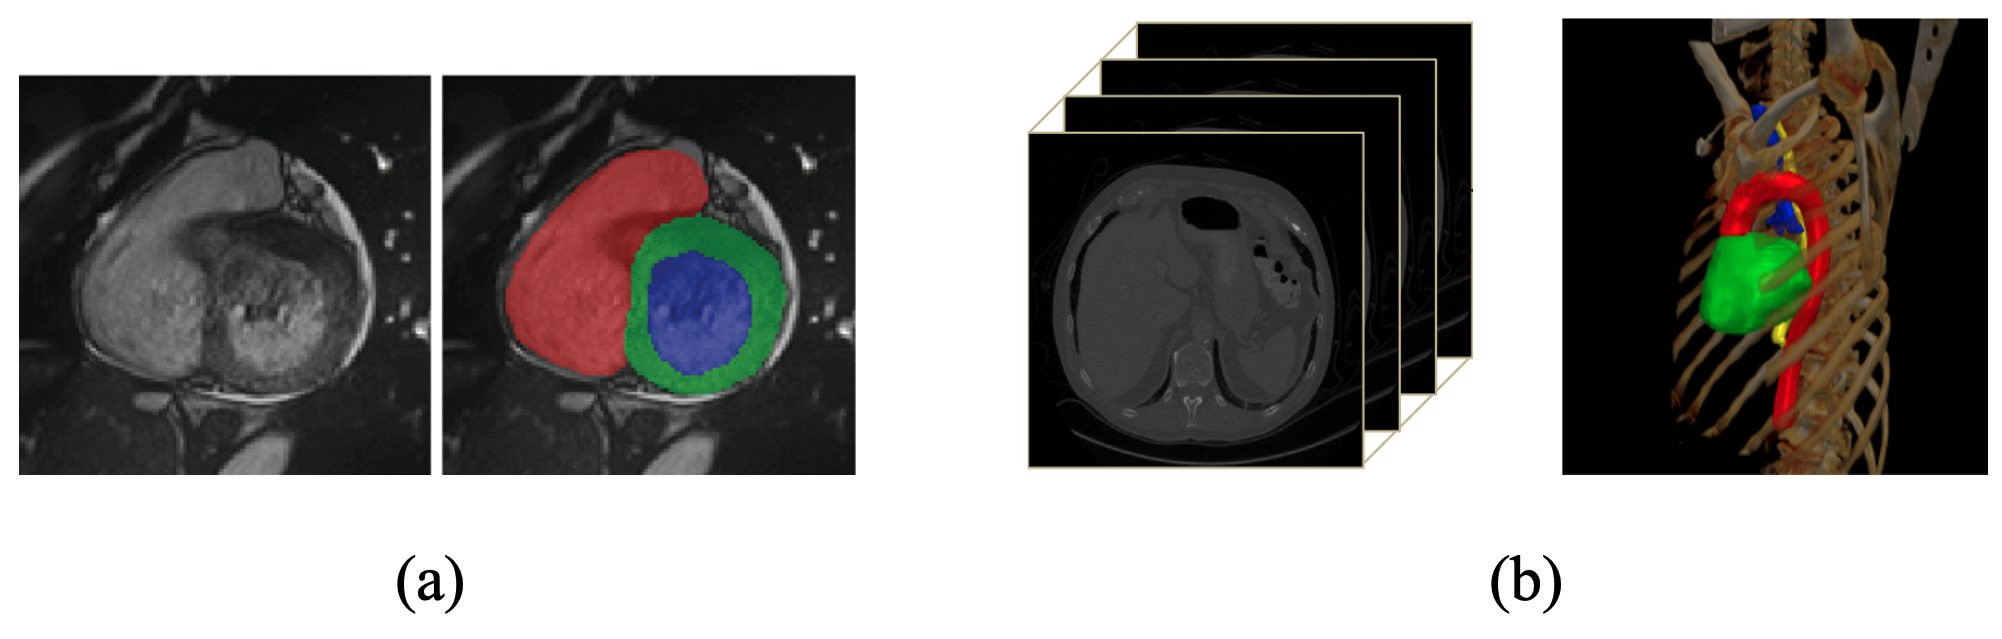
\includegraphics[width=1.0\textwidth]{img/c3/c3_1.png}
        \bicaption{医学图像的语义分割任务示例。左侧为二维图像与分割标签,右侧为三维图像(由一系列连续的二维图像组成)及其标签。}
        {Examples of medical image semantic segmentation. (a) 2D image and its segmentation label. (b) 3D image and its segmentation label.}
        \label{c3_fig1}
    \end{figure*}

    \begin{figure*}[t!]
        \centering 
        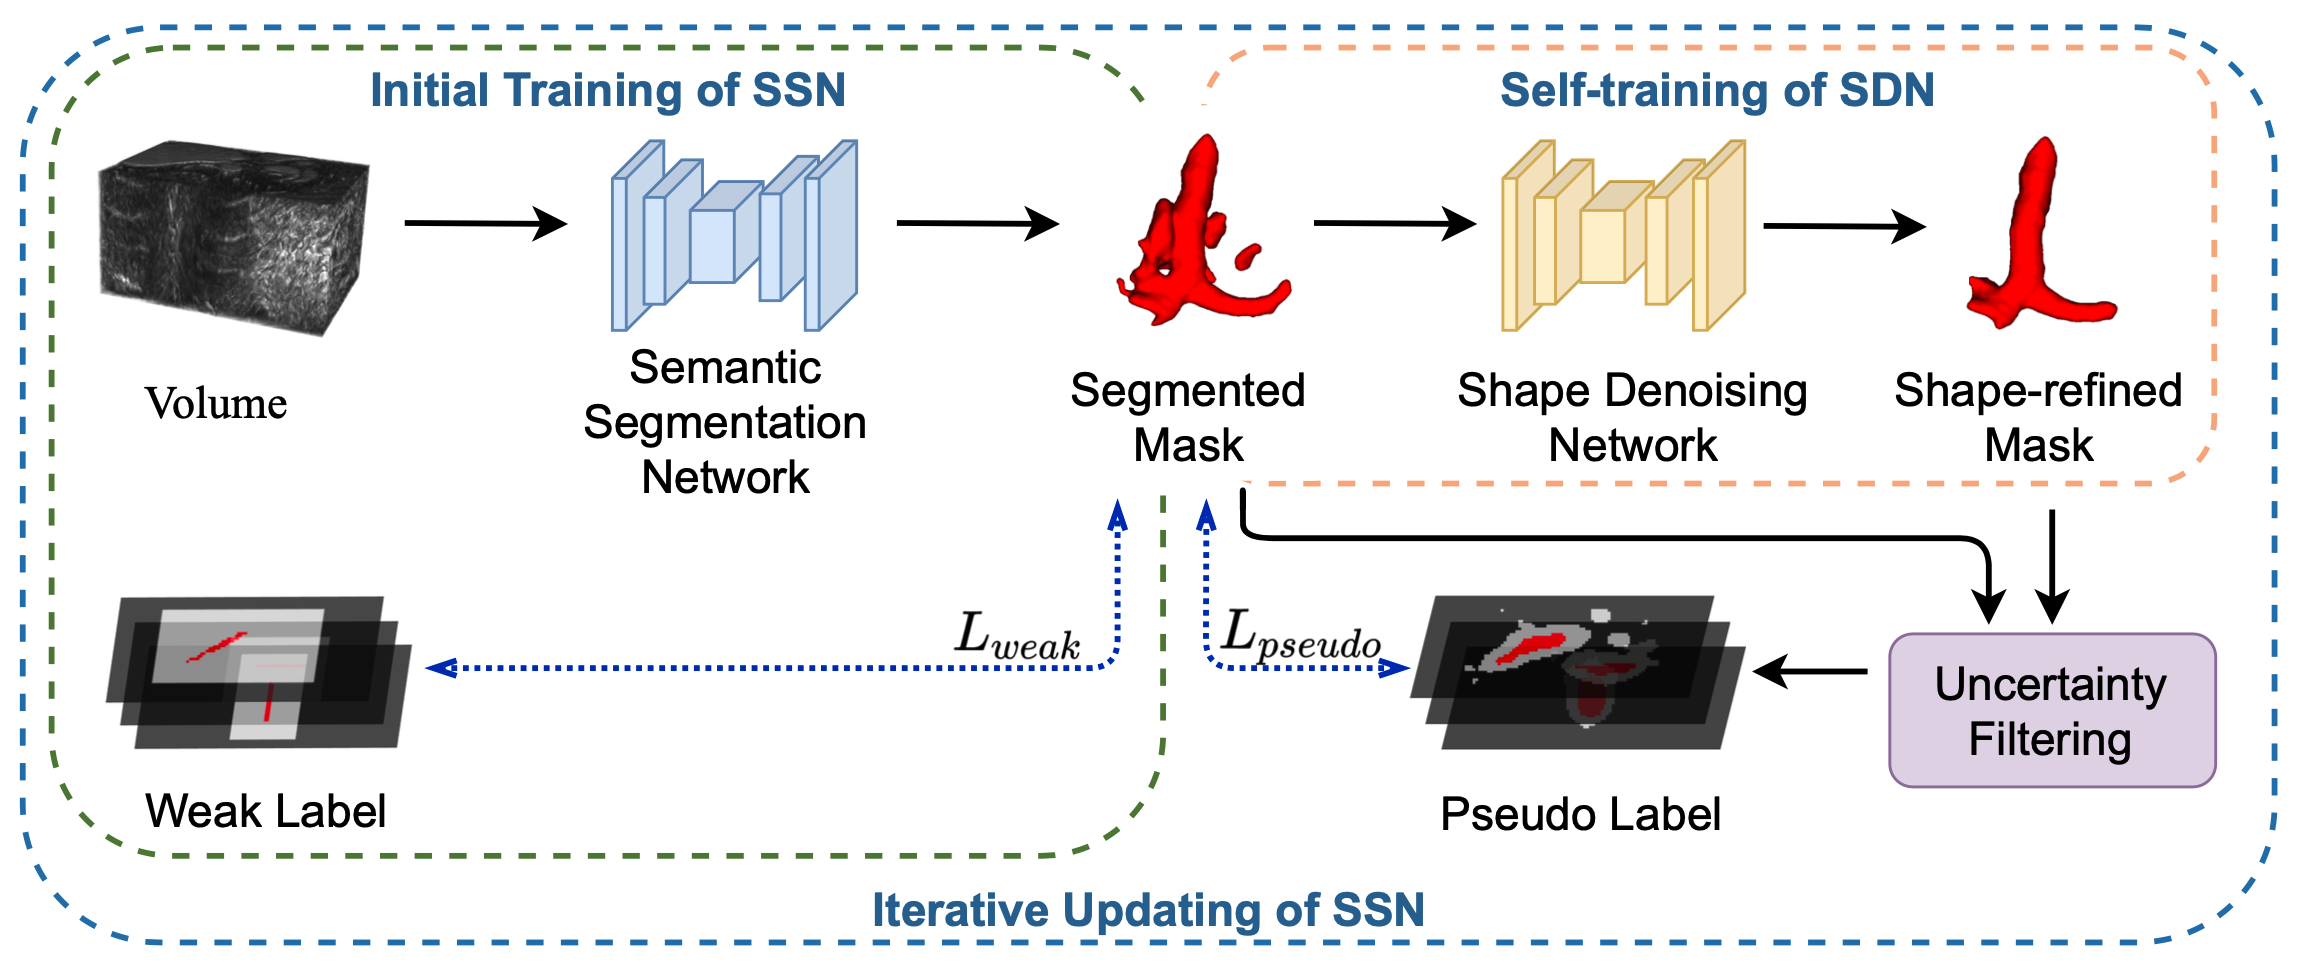
\includegraphics[width=1.00\textwidth]{img/c3/b_model_shape.png}
        \bicaption{弱监督语义分割模型概览。我们的模型由两个主要模块组成:语义分割网络和形状去噪网络。语义分割网络从输入的体积图像中预测出一个初始的分割掩膜,并由其后形状去噪网络进一步完善,作为最终输出。我们采用一种迭代训练的方法来训练模型。}
        {The overview of our method. Our model consists of two main modules: Semantic Segmentation Network (SSN) and Shape Denoising Network (SDN). Our SSN predicts an initial segmented mask from the input volumetric image, which is further refined by our SDN as final output. To train our model, we propose an iteraitve learning strategy.}
        \label{fig:model}
    \end{figure*}


\section{模型设计}
在本节我们详细介绍模型中的两个主要模块:语义分割网络和形状去噪网络。

\textbf{语义分割网络} \quad 语义分割网络 $\mathcal{F}_{SSN}$ 用来产生一个初始的粗分割掩膜,它将一个体积图像 $\mathbf{I}$ 作为输入,并输出一个概率图 $\mathbf{P}_s \in [0,1]^{H\times W\times D}$,表示每个像素属于前景的置信度。由 $\mathbf{P}_s$ 我们可以得出初始的前景分割掩膜 $\mathbf{M}_s$:
\begin{align}
    \mathbf{P}_s = \mathcal{F}_{SSN} (\mathbf{I}; \Theta), \mathbf{M}_s = \mathds{1} (\mathbf{P}_s > 0.5)
\end{align}
其中 $\Theta$ 表示 $\mathcal{F}_{SSN}$ 的参数,而 $\mathds{1}(\cdot)$ 是一个指示函数。
我们用 nnU-Net~\citep{isensee2019automated} 来实例化我们的语义分割网络,它是医学图像语义分割的最先进而广泛的模型结构。
% 可扩展:将 模型的具体设计可再讲一段,从附录 C 里取出。


\textbf{形状去噪网络} \quad 我们设计了一个形状去噪网络 $\mathcal{F}_{SDN}$ 来编码一个统一的形状先验,然后应用于初始的粗分割掩膜上进行形状改进。形状去噪网络的思想借鉴自去噪自编码器\citep{vincent2010stacked}和增强自编码器\citep{Sundermeyer_2018_ECCV}。去噪自编码器将图像编码为对噪声不敏感的隐向量,以表示原始的干净图像。增强自编码器产生输入图像中物体的方向编码,而对其他变换和环境条件具有不变性。与这些旨在为图像或物体方向提供代表性向量表征的方法不同,我们的目标是将输入的粗分割掩膜中恢复为干净而完整的形状。
给定语义分割网络输出的初始掩膜 $\mathbf{M}_s$,我们的形状去噪网络隐式地施加了自学习的形状先验约束,并输出一个干净的形状改进的分割掩膜:
\begin{align}
    \mathbf{P}_d = \mathcal{F}_{SDN} (\mathbf{M}_s; \Omega), \mathbf{M}_d = \mathds{1} (\mathbf{P}_d > 0.5)
\end{align}
其中 $\Omega$ 表示 $\mathcal{F}_{SDN}$ 的参数。由于我们的输出目标是最终的分割掩膜,而不是隐向量表示,我们的 $\mathcal{F}_{SDN}$ 采用了与 $\mathcal{F}_{SSN}$ 相同的 U-Net 结构,这种设计使得形状去噪网络在中间瓶颈层也保持较大的空间分辨率,并包含跳跃连接以捕捉更多的分割细节。

\section{弱标注策略}
为了更好地利用物体掩膜的空间连续性并促进形状上下文的学习,我们为三维体积分割任务设计了一个稀疏的弱标注策略。
标注方案包含两个方面,切片选择和混合式标签策略。三维图像由一系列连续的二维切片组成,但我们不需要逐切片地标注,而是对切片选择性标注。对切片选择方法,我们先选择标注每个前景物体的起始和结束的切片,因为它们包括 $z$ 轴上的重要边界信息。除了这两个切片,我们还随机标注它们之间切片的一个子集。在这项工作中,我们研究了多个标注比例设定,分别是 10\%、30\%、50\%和100\%的前景切片标注比例。
另一方面,我们为二维切片设计了一种混合式标签,它包括在前景物体区域的一条长轴涂鸦和一个包围所有前景像素的松散边界框。具体来说,对于长轴涂鸦,标注者只需在前景物体内部的边界附近点击两个点,就可以根据两段点自动形成一条线。对于松散的边界框,标注者只需要点击位于左上角和右下角的两个点,就可以自动形成一个矩形框。
值得注意,我们的混合式标签并不需要对边界点进行精确的定位,而只需要标注者大致指出前景的内部和外部区域。与传统的涂鸦式标签或紧致的边界框相比,混合式标签可以提供丰富的背景信息和粗略的定位,以及前景像素标签,而每个 2D 切片只需四个标注点。为了模拟我们的弱标注策略,我们从全掩膜中生成混合式标签。图~\ref{fig:weak_annotation}中显示了一些例子。
% 可扩展:将弱标签在附录B中的两段内容拿出来扩展。

    \begin{figure*}[tbp]
        \centering 
        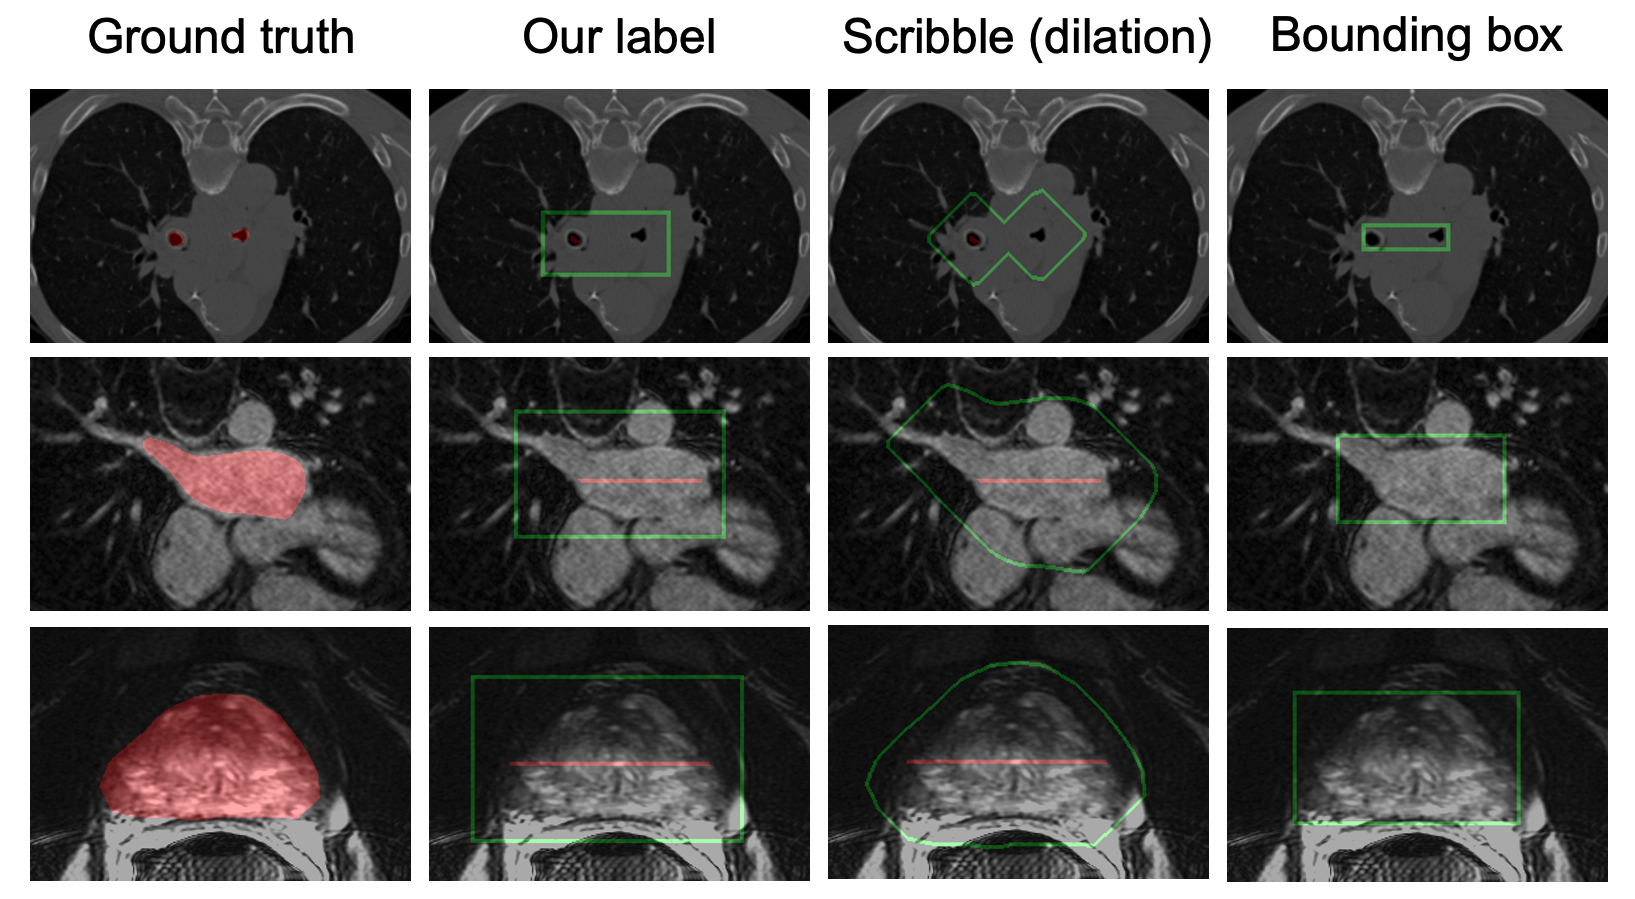
\includegraphics[width=1.0\textwidth]{img/c3/c_weak_annotation2.png}
        \bicaption{不同标注方法的示意图,分别在气管(第一行)、左心房(第二行)和前列腺(第三行)的图像上展示。第一列为精确的全标注,第二列为我们的混合式标注方法,第三列是涂鸦式标注(由前景区域膨胀操作模拟生成),第四列是紧致的边界框标注。}
        {We show different annotations for trachea (first row), left atrium (second row) and prostate (last row). Four rows show groundtruth, our hybrid label, scribble and bounding box, respectively. Scribble (dilation) denotes generated scribble by foreground mask dilation.}
        \label{fig:weak_annotation}
    \end{figure*}

\section{模型训练}
为了有效地训练提出的模型,我们采用了一个迭代学习框架,它迭代地生成伪标签和更新模型参数。为了生成初始伪标签,我们首先初始化训练模型中的语义分割网络和形状去噪网络。然后,我们结合语义分割网络和形状去噪网络的输出,并通过不确定性过滤机制来计算生成伪标签。两个输出的结合是为了消除噪声并在模型更新中引入学到的形状先验。
接下来,我们依次介绍语义分割网络的训练、自学习的形状去噪网络的训练、不确定性过滤机制的伪标签生成,以及最终的模型更新。

\paragraph{训练语义分割网络}
我们首先在弱标签上训练语义分割网络,以提供初始分割掩膜。初始掩膜会作为形状去噪网络的重要训练信息。
给定输入图像和相应的弱标签,我们使用有标签像素上的加权交叉熵来训练语义分割网络:
\begin{align}
    \mathcal{L}_{SSN} (\Theta) = \mathcal{L}_{wce} (\mathbf{P}_s, \mathbf{Y})
\end{align}
在我们的混合式标签中,边界框外的区域全部可视为背景像素,而前景只有涂鸦式标签覆盖的像素。由于弱标签中前景和背景的极大不平衡,我们在损失函数中采用了自动加权策略,来平衡前景和背景的影响。实验表明,与固定的加权比例相比,我们的自动加权策略更加稳定,对不同的数据集有更好的泛化性。
具体来说,对于每个有 $N_b$ 个有标签背景像素和 $N_f$ 个有标签前景像素,我们计算损失为
\begin{align}
    (\frac{1}{N_b} \sum^{N_b}_{i} l_i + \frac{1}{N_f} \sum^{N_f}_{j} l_j) / 2
\end{align}
其中 $l_i$ 表示第 $i$ 个像素的交叉熵损失。

\paragraph{自训练的形状去噪网络}
不同于之前的去噪模型学习方法,我们用自学习的策略来训练形状去噪网络。\citet{vincent2010stacked} 对输入图像应用人工的随机噪声增强,并重建对应的干净图像目标。\citet{Sundermeyer_2018_ECCV} 提出了一种域随机化技术,以模拟真实相机捕捉的环境和传感器变化。他们利用这种技术来增强输入合成图像,并重建除方向外其他因素不变性的图像。

对我们的问题,一个重要的区别是,没有用于自学习的完整掩膜标签。即没有可用的训练目标标签,这里是形状完整的标签。
一个可能的解决方案是使用数字合成的形状模型,但对不同的数据集可能有很大的域差距,特别是对医学分割中的掩膜。为了避免这种域差距,我们提出了一个自学习策略:首先用弱监督分割模型中的语义分割网络提取出自学习的形状表示,然后用这样的形状表示来训练形状去噪网络。其基本假设是,我们初训练的语义分割网络能够在训练集中的某些实例上产生高于平均水平的分割掩码,因此能够提供形状质量较好的分割掩膜,来帮助改善其他形状质量较差的掩膜。为此,我们首先计算训练集中每个 $\mathbf{P}_s$ 的平均前景概率,作为每个分割掩膜 $\mathbf{M}_s$ 的置信度,然后选取置信度最高的分割掩膜作为我们自学的表示 $\mathbf{M}^*$ 来训练形状去噪网络。

形状去噪网络的作用是去除形状层面的噪声,为了训练这种能力,我们不是在输入掩膜中加入通常的随机噪声,而是根据初始化的语义分割网络输出的错误模式的观察,特别设计形状层面的噪声增强方法。
我们将初始分割掩膜的典型错误模式总结为三类。
\begin{enumerate}
    \item 过度平滑的区域。这是由于边缘区域的监督信号较少,模型无法区分准确边缘所致。
    \item 表面错误附着的斑块。仅根据视觉特征,容易把其他相近的区域也预测为目标物体的一部分。
    \item 轴向上超出前景起始和结束切片的多余预测。根据相近的视觉特征和连续性,容易产生错误的轴向物体延长。
\end{enumerate}
这些形状错误模式主要是因为在弱标签中没有明确的边界监督,而邻近的物体区域可能与目标物体有相似的强度或纹理特征。

为了使我们的形状去噪网络具备处理上述错误的能力,我们设计了三种相应的噪声增强操作。(1) 形态学的闭操作;(2) 形态学的膨胀;(3) 边缘切片的形状延伸。例子如图~\ref{fig:shape_aug}所示。
    \begin{figure*}[tbp]
        \centering 
        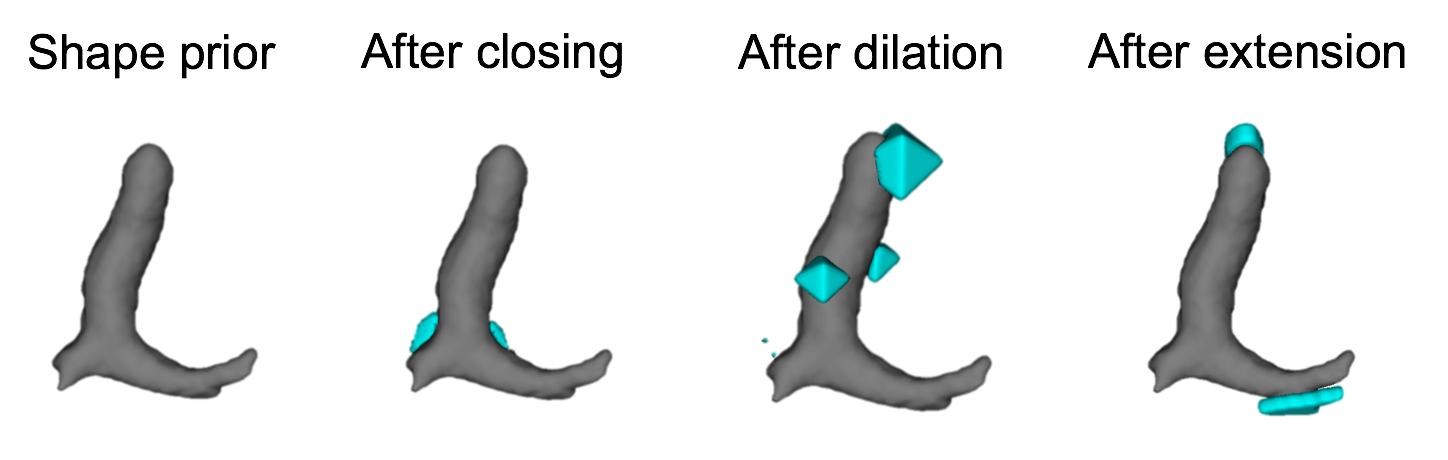
\includegraphics[width=1.0\textwidth]{img/c3/b_shape_aug2.png}
        \bicaption{气管分割上,我们自学习的形状表示和对应的噪声增强的示意图。}
        {An example of our self-taught shape representation and corresponding augmentation effect on trachea.}
        \label{fig:shape_aug}
    \end{figure*}
为了充分扩充形状去噪网络的训练数据集,我们还应用了空间变换,包括旋转、平移和缩放。这样可以捕捉丰富的位置和尺寸变化,有助于学习隐式的形状流形。我们将自学习的形状表征M∗增强为M∗,并训练我们的SDN来重建具有交叉熵损失的干净面具M∗。
我
们应用空间转换,包括旋转、平移和缩放,以捕捉丰富的位置和尺寸变化,这有助于学习潜在的形状流形。我们将自学的形状表征 $\mathbf{M}^*$ 增强为 $\mathbf{\hat{M}}^*$ 作为输入,并训练形状去噪网络来重建干净的掩膜 $\mathbf{M}^*$:
\begin{align}
    \mathcal{L}_{SDN} (\Omega) = \mathcal{L}_{ce} (\mathcal{F}_{SDN} (\mathbf{\hat{M}}^*; \Omega), \mathbf{M}^*)
\end{align}

\paragraph不确定性过滤}
为了利用自学习的形状先验来进一步改进我们的模型并去除预测标签的噪声,我们设计一个不确定性过滤机制,从语义分割网络和形状去噪网络的概率预测中生成伪掩膜标签。具体地说,我们首先计算语义分割网络和形状去噪网络各自输出的分割掩膜,对二者取交集,然后根据语义分割输出中P s的每个像素的确定性,

不确定性过滤 为了结合自学的形状先验来进一步改善我们的模型并去除噪音,我们用一个简单的不确定性过滤机制从SSN和SDN的预测中生成伪掩码。具体来说,我们首先计算SSN的分割面具和SDN的形状重构面具的交集,然后根据语义分割输出 $\mathbf{P}_s$ 中每个像素的置信度,应用基于不确定性的过滤。我们为前景($\mathbf{Y}_{fg}$)和背景($\mathbf{Y}_{bg}$)独立计算伪标签掩膜,
\begin{align}
    \mathbf{Y}_{fg} &= \mathbf{M}_s * \mathbf{M}_d * \mathds{1} (\mathbf{P}_s > \sigma_{fg})
\end{align}
\begin{align}
    \mathbf{Y}_{bg} = (1-\mathbf{M}_s) * (1-\mathbf{M}_d) * \mathds{1} (\mathbf{P}_s < \sigma_{bg})
\end{align}
其中 $\sigma_{fg}$ 和 $\sigma_{bg}$ 是前背景各自的不确定性阈值。
最后的伪标签 $\mathbf{Y}_p$ 结合了 $\mathbf{Y}_{fg}$ 和 $\mathbf{Y}_{bg}$,
\begin{align}
    \mathbf{Y}_p &= \mathds{1}(\mathbf{Y}_{fg} = 1) + u * \mathds{1}(\mathbf{Y}_{fg} = 0) * \mathds{1}(\mathbf{Y}_{bg} = 0)
\end{align}
其中无标签的像素设置为 $u$。

\paragraph{模型更新}
得到生成的伪标签 $\mathbf{Y}_p$,我们通过最小化两项加权的交叉熵损失来更新模型参数 $\Theta$ :分割输出概率 $\mathbf{P}_s$ 相对于原始的弱标签和生成的伪标签,
\begin{align}
    \mathcal{L} (\Theta) = \lambda_w \mathcal{L}_{wce} (\mathbf{P}_s, \mathbf{Y}) + \lambda_p \mathcal{L}_{wce} (\mathbf{P}_s, \mathbf{Y}_p)
\end{align}
其中 $\lambda_w$ 和 $\lambda_p$ 是各自相应的损失权重。
在迭代学习中,我们冻结了形状去噪网络的参数 $\Omega$。这是根据实验观察,更新 $\Omega$ 并不能带来进一步的改善。主要因为我们自学习的形状表示已经有相对较好的质量,而且设计的形状噪声增强足够充分,可以捕捉到各种错误模式。


\section{实验}
我们在三个公开的基准上评估了我们的方法,它们分别具有不同的形状,包括 SegTHOR\citep{trullo2019multiorgan}中的气管、心房分割挑战赛中的左心房和 PROMISE12\citep{Litjens2014EvaluationOP}中的前列腺。在每个数据集上,我们与使用不同弱标签的最先进的方法进行比较。
下面我们首先在~\ref{sec:dataset}节介绍数据集信息,在~\ref{sec:detail}节介绍实现细节。然后,我们在~\ref{sec:res1}节和~\ref{sec:res2}节分别介绍了与其他方法比较的定量结果和定性结果,最后在~\ref{sec:detail}节中介绍了完整的消融实验对比。
% 此外,我们在附录F中对我们的SDN进行了进一步的分析,以更好地理解形状去噪机制,并在附录G中讨论了我们的失败案例和潜在的未来工作。

\subsection{实验数据集} \label{sec:dataset}

\paragraph{SegTHOR挑战赛}
SegTHOR挑战赛\footnote{https://competitions.codalab.org/competitions/21145}\citep{trullo2019multiorgan}由60个胸部CT扫描图组成,来自被诊断为肺癌或霍奇金淋巴瘤的患者。这个数据集的所有扫描图像的尺寸为$512\times512\times(150-284)$,切面内的间距从 0.90 毫米到 1.37 毫米不等,切面间的间距从 2 毫米到 3.7 毫米。我们对数据集划分如下:将 40 份公开可用的扫描图分成 30 份作为训练,10 份用于验证,并将 20 份测试数据的结果上传官方网页在线评估。这个数据集包含四个器官:心脏、主动脉、气管和食管。我们在气管上进行实验,因为它更具有挑战性和代表性的器官形状。

\paragraph{左心房数据集}
左心房数据集来自2018心房分割挑战赛\footnote{http://atriaseg2018.cardiacatlas.org/}。它包含100对三维钆增强的 MR 成像扫描(GE-MRIs)和对应的左心房分割掩膜。所有扫描都是各向同性的,其间距为 $0.625\times0.625\times0.625 mm^{3}$。每个病人的 MRI 图像的切面分辨率不同,而 Z 轴上都是 88 张切面。我们将 100 个扫描图分成 60 个用于训练,20 个用于验证,20 个用于测试。

\paragraph{PROMISE12挑战赛}
PROMISE12挑战赛\footnote{https://promise12.grand-challenge.org}\citep{Litjens2014EvaluationOP}包含 50 个横向 T2 加权 MR 图像,采用多种扫描协议,其分割目标前列腺位于图像的中央区域。这个数据集中的所有病例都是各向异性的,间距$2\times0.27\times0.27 mm^{3}$ 到 $4\times0.75\times0.75 mm^{3}$。我们采用与\citet{kervadec2020bounding}相同的设置,将 50 个扫描图分成 40 个用于训练,10 个用于验证。由于在线测试已不再支持,我们报告验证部集上的结果。

\subsection{实现细节} \label{sec:detail}

有些数据集(如SegTHOR)中的三维图像尺寸过大,直接作为模型输入需要大量的计算资源和时间,十分低效。
为了让目标物体的三维图像适应分割模型的输入,我们采用了基于弱标签的裁剪数据的预处理方法。具体来说,我们首先将体积图像重新取样到相同的体素间距,然后根据它们的中心对齐所有的训练样本,并将它们扩充到相同的大小,最后从所有样本中裁剪出一个统一的立方体,它是所有弱标注像素的交集所构成立方体的 1.2 倍。所有在我们的松散边界框外的像素,以及在起点和终点切片之外的像素,都被视为背景标签。

对于我们在训练形状去噪网络时的噪声增强,详细的处理如下。(1) 比操作。我们对目标形状应用标准的形态学闭操作,即首先进行膨胀,然后进行腐蚀。闭操作提供了过度平滑的掩膜,这是气管和左心房的一个常见错误。(2) 膨胀。我们首先随机选择一个靠近掩膜边界的点作为中心,然后用一个范围内的随机迭代次数来膨胀。对于各向异性的数据集如前列腺,我们基于二维切片膨胀,而对于各向同性的数据集,我们采用三维膨胀。(3) 边缘切片的形状延伸。我们通过在 Z 轴上复制一些前景起始或结束的切片来延伸掩模。默认情况下,我们采用概率为 0.2 的随机空间变换,以丰富形状变化。

训练方法如下。参考\citet{isensee2019automated},我们采用相同的图像增强方法和深度监督模型方法训练,批大小为2。我们使用 SGD 优化器来训练。
对于初始化,我们用 1e-2 的初始学习率训练语义分割网络,并在多项式衰减策略下将其衰减到 1e-3,持续 200 轮。为了训练形状去噪网络,我们使用 1e-2 的固定学习率训练 100 轮。在迭代学习中,我们对不同的数据集使用不同的训练参数。在不确定性过滤中,对于每个体积图像,我们首先对预测的分割置信图 $\mathbf{P}_s$ 中的像素按置信度进行排序,然后设置前景不确定性阈值 $\sigma_{fg}$ ,以过滤掉置信度较低的部分。这个前景过滤比例 $\sigma_{fg}$ 对气管设为70\%,对左心房和前列腺的设为50\%。相应地,每个数据集的背景过滤比例 $\sigma_{bg}$ 被设定为  $2\sigma_{fg}$。
在模型参数更新中,对于气管,我们将损失权重($\lambda_w$, $\lambda_p$)设置为(1, 100),并以 1e-3 的学习率再训练我们的模型最多 300 次。对于前列腺,我们设定($\lambda_w$, $\lambda_p$)为(0.1, 10),学习率为 1e-2。对于左心房,我们设定($\lambda_w$, $\lambda_p$)为(0.1, 10),学习率为1e-3。


\subsection{定量结果} \label{sec:res1}



    % \begin{table}[t!]
    %     \centering    
    %     \resizebox{\textwidth}{!}{
    %         \begin{tabular}{c|c|c c c c |c c c c}
    %             \toprule
    %             \multirow{2}{*}{Method} & \multirow{2}{*}{Annotation} & \multicolumn{4}{c|}{Trachea (Test)} & \multicolumn{4}{c}{Left Atrium (Test)}    \\ 
    %             &                        & 100\% & 50\% & 30\% & 10\%  & 100\% & 50\% & 30\% & 10\%                                         \\ \midrule
    %             nnU-Net~\cite{isensee2019automated}     & Full label        & \multicolumn{4}{c|}{89.74}           & \multicolumn{4}{c}{92.63} \\ \cmidrule{1-10}
    %             BoxPrior\cite{kervadec2020bounding}    & Box  & 79.82  & 48.78  & -- & -- & 83.93  & 83.51  & 81.86 & --           \\
    %             KernelCut\cite{tang2018regularized}   & Scribble* & 84.39  & 83.44  & 82.77  & 67.78 & 78.97  & 76.71  & 74.42  & 64.93            \\
    %             Ours & Scribble* & 84.61 & 83.88 & 83.37 & 81.82 & 85.61 & 84.11 & 83.26 & 83.11 \\
    %             KernelCut\cite{tang2018regularized}   & Hybrid & 84.74 & 83.55	& 83.38	& 76.43 & 77.54	& 76.72	& 73.64	& 67.27            \\
    %             Ours        & Hybrid    & \textbf{85.54} & \textbf{83.97} & \textbf{83.78} & \textbf{83.19} & \textbf{86.31} & \textbf{86.25} & \textbf{83.81} & \textbf{83.41}                                \\
    %             \bottomrule
    %         \end{tabular}
    %     }
    %     \bicaption{在气管和左心房测试集上的定量结果。表中数值的单位是 Dice [\%]。“--”表示对应的方法未能预测有意义的前景区域。}
    %     {Quantitative results on the test splits of trachea and left atrium. All presented numbers are in Dice [\%]. '--' under 10\% denotes that BoxPrior failed in predicting any foreground.}
    %     \label{tab:test_result}
    % \end{table}


\subsection{定性结果} \label{sec:res2}




\subsection{消融实验} \label{sec:ablate}



\section{实验}
